\documentclass[11pt,a4paper]{article}
\usepackage[T1]{fontenc}
\usepackage[utf8]{inputenc}
\usepackage{palatino}
\usepackage[margin=2.5cm]{geometry}
\usepackage{xcolor}
\usepackage{tikz}
\usepackage{amsmath, amssymb}
\usepackage{bm}
\usepackage[most]{tcolorbox}
\usepackage{pifont}
\usetikzlibrary{positioning, arrows.meta, shapes.geometric, shapes.symbols, decorations.pathmorphing, calc, chains}

% Couleurs
\definecolor{atmcolor}{RGB}{70,130,180}
\definecolor{chk2color}{RGB}{255,140,0}
\definecolor{cdc25color}{RGB}{220,20,60}
\definecolor{cdk1color}{RGB}{50,205,50}
\definecolor{cyclincolor}{RGB}{147,112,219}
\definecolor{phosphocolor}{RGB}{255,200,0}
\definecolor{stopcolor}{RGB}{220,50,50}
\definecolor{gocolor}{RGB}{50,205,50}

\begin{document}

\begin{center}
{\LARGE\bfseries\color{atmcolor} La cascade de signalisation ATM}\\[0.5cm]
{\large Blocage du complexe CDK1/Cycline B et arrêt du cycle cellulaire}
\end{center}

\vspace{0.5cm}

%==============================================================================
% SECTION 1 : Explication simple
%==============================================================================
\section{Comprendre la phrase}

\begin{tcolorbox}[colback=blue!5, colframe=atmcolor, title=\textbf{La phrase à expliquer}]
\textit{``Une fois activée, ATM déclenche une cascade de phosphorylations qui aboutit au blocage du complexe CDK1/Cycline B, le "moteur" de l'entrée en mitose.''}
\end{tcolorbox}

\subsection{Décomposition des termes}

\begin{itemize}
    \item \textbf{ATM activée} : La protéine ATM a détecté des cassures double-brin et s'est autophosphorylée
    \item \textbf{Cascade de phosphorylations} : Série de réactions en chaîne où chaque protéine en active une autre en lui ajoutant un phosphate
    \item \textbf{CDK1/Cycline B} : Complexe protéique qui déclenche l'entrée en mitose (division cellulaire)
    \item \textbf{``Moteur''} : Sans ce complexe actif, la cellule ne peut pas entrer en mitose
\end{itemize}

%==============================================================================
% FIGURE 1 : La cascade simplifiée
%==============================================================================
\section{La cascade de signalisation}

\begin{figure}[h!]
\centering
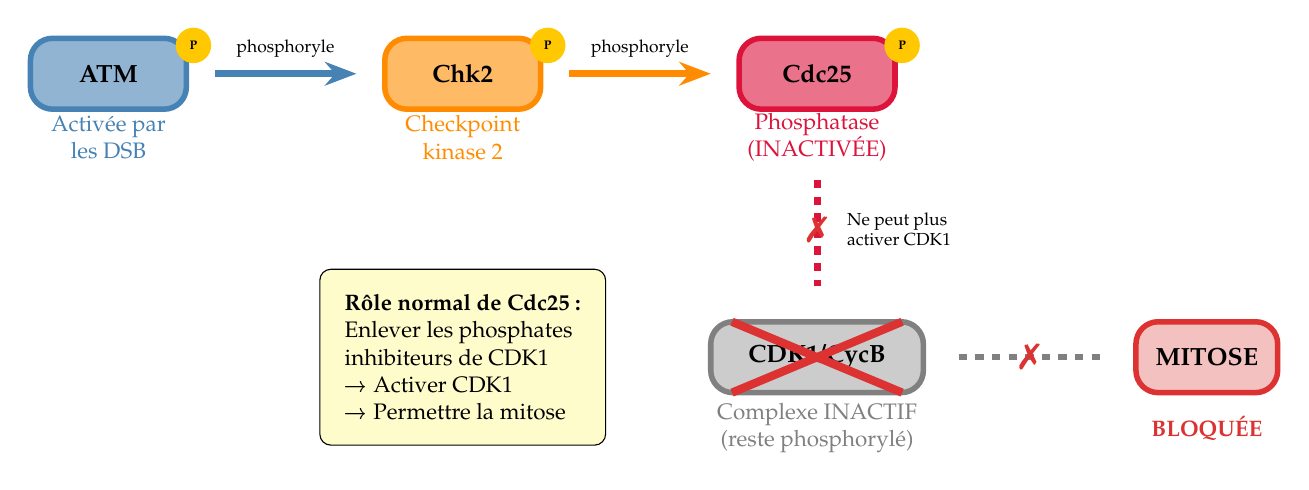
\begin{tikzpicture}[
    scale=0.9, 
    transform shape,
    protein/.style={rectangle, rounded corners=8pt, minimum width=2.2cm, minimum height=1cm, line width=2pt, font=\bfseries, align=center},
    arrow/.style={-{Stealth[length=4mm, width=3mm]}, line width=2.5pt},
    phospho/.style={circle, fill=phosphocolor, minimum size=0.5cm, font=\tiny\bfseries}
]
    
    % === ATM ===
    \node[protein, fill=atmcolor!60, draw=atmcolor] (atm) at (0, 0) {ATM};
    \node[phospho] at (1.2, 0.4) {P};
    \node[font=\small, atmcolor, align=center] at (0, -0.9) {Activée par\\les DSB};
    
    % Flèche ATM → Chk2
    \draw[arrow, atmcolor] (1.5, 0) -- (3.5, 0);
    \node[font=\scriptsize, above] at (2.5, 0.1) {phosphoryle};
    
    % === Chk2 ===
    \node[protein, fill=chk2color!60, draw=chk2color] (chk2) at (5, 0) {Chk2};
    \node[phospho] at (6.2, 0.4) {P};
    \node[font=\small, chk2color, align=center] at (5, -0.9) {Checkpoint\\kinase 2};
    
    % Flèche Chk2 → Cdc25
    \draw[arrow, chk2color] (6.5, 0) -- (8.5, 0);
    \node[font=\scriptsize, above] at (7.5, 0.1) {phosphoryle};
    
    % === Cdc25 ===
    \node[protein, fill=cdc25color!60, draw=cdc25color] (cdc25) at (10, 0) {Cdc25};
    \node[phospho] at (11.2, 0.4) {P};
    \node[font=\small, cdc25color, align=center] at (10, -0.9) {Phosphatase\\(INACTIVÉE)};
    
    % Flèche Cdc25 --X--> CDK1
    \draw[line width=2.5pt, cdc25color, dashed] (10, -1.5) -- (10, -3);
    \node[font=\Large, stopcolor] at (10, -2.2) {\ding{55}};
    \node[font=\scriptsize, right, align=left] at (10.3, -2.2) {Ne peut plus\\activer CDK1};
    
    % === CDK1/CycB (bloqué) ===
    \node[protein, fill=gray!40, draw=gray, minimum width=3cm] (cdk1) at (10, -4) {CDK1/CycB};
    \node[font=\small, gray, align=center] at (10, -5) {Complexe INACTIF\\(reste phosphorylé)};
    
    % Croix sur CDK1
    \draw[stopcolor, line width=3pt] (8.8, -3.5) -- (11.2, -4.5);
    \draw[stopcolor, line width=3pt] (8.8, -4.5) -- (11.2, -3.5);
    
    % === Flèche vers MITOSE bloquée ===
    \draw[line width=2pt, gray, dashed] (12, -4) -- (14, -4);
    \node[font=\Large, stopcolor] at (13, -4) {\ding{55}};
    
    % === MITOSE ===
    \node[protein, fill=stopcolor!30, draw=stopcolor, minimum width=2cm] (mitose) at (15.5, -4) {MITOSE};
    \node[font=\small\bfseries, stopcolor] at (15.5, -5) {BLOQUÉE};
    
    % === Encadré explicatif ===
    \node[draw, rectangle, rounded corners, fill=yellow!20, inner sep=10pt, font=\small, align=left] at (5, -4) {
        \textbf{Rôle normal de Cdc25 :}\\
        Enlever les phosphates\\
        inhibiteurs de CDK1\\
        → Activer CDK1\\
        → Permettre la mitose
    };
    
\end{tikzpicture}
\caption{\textbf{La cascade ATM $\rightarrow$ Chk2 $\rightarrow$ Cdc25 $\dashv$ CDK1.} ATM activée phosphoryle Chk2, qui phosphoryle Cdc25. Cdc25 phosphorylée est inactive et ne peut plus activer CDK1/Cycline B. Sans CDK1 actif, la cellule ne peut pas entrer en mitose.}
\end{figure}

%==============================================================================
% FIGURE 2 : CDK1/Cycline B = Le moteur
%==============================================================================
\section{CDK1/Cycline B : Le ``moteur'' de la mitose}

\begin{figure}[h!]
\centering
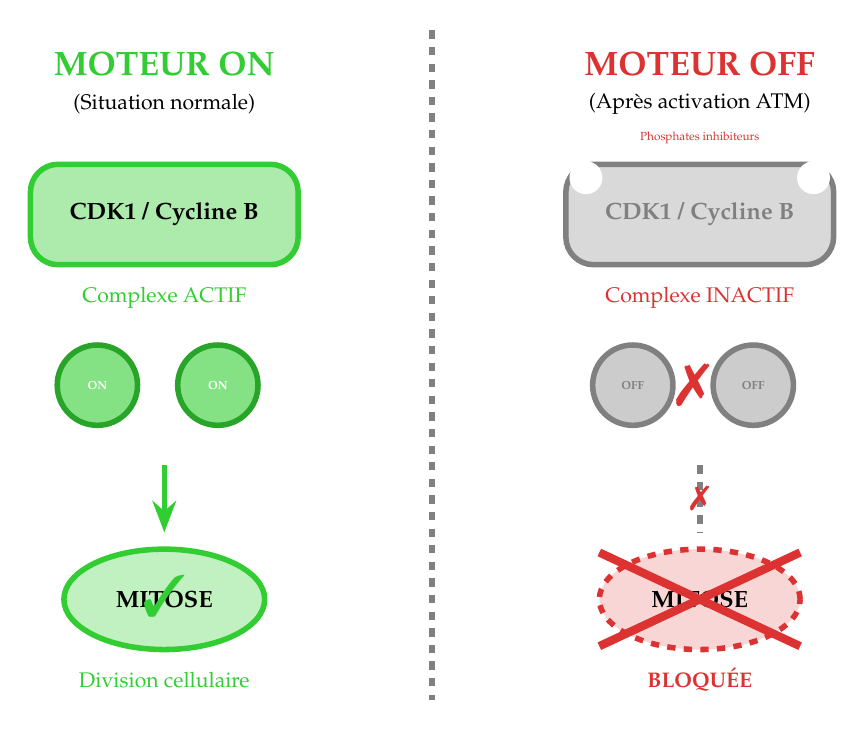
\begin{tikzpicture}[scale=0.85, transform shape]
    
    % === TITRE GAUCHE : Moteur ON ===
    \node[font=\Large\bfseries, gocolor] at (-4, 4) {MOTEUR ON};
    \node[font=\small] at (-4, 3.4) {(Situation normale)};
    
    % CDK1/CycB actif
    \draw[fill=gocolor!40, rounded corners=10pt, line width=2pt, draw=gocolor] (-6, 1) rectangle (-2, 2.5);
    \node[font=\bfseries] at (-4, 1.75) {CDK1 / Cycline B};
    \node[font=\small, gocolor] at (-4, 0.5) {Complexe ACTIF};
    
    % Engrenages tournants (représentés par des cercles)
    \node[circle, fill=gocolor!60, minimum size=1.2cm, draw=gocolor!80!black, line width=2pt] at (-5, -0.8) {};
    \node[circle, fill=gocolor!60, minimum size=1.2cm, draw=gocolor!80!black, line width=2pt] at (-3.2, -0.8) {};
    \node[font=\tiny\bfseries, white] at (-5, -0.8) {ON};
    \node[font=\tiny\bfseries, white] at (-3.2, -0.8) {ON};
    
    % Flèche vers mitose
    \draw[-{Stealth[length=4mm]}, line width=2pt, gocolor] (-4, -2) -- (-4, -3);
    
    % Mitose OK
    \node[ellipse, fill=gocolor!30, draw=gocolor, line width=2pt, minimum width=3cm, minimum height=1.5cm] at (-4, -4) {\textbf{MITOSE}};
    \node[font=\small, gocolor] at (-4, -5.2) {Division cellulaire};
    
    % Checkmark
    \node[font=\Huge, gocolor] at (-4, -3.95) {\ding{51}};
    
    % === SÉPARATEUR ===
    \draw[line width=2pt, gray, dashed] (0, 4.5) -- (0, -5.5);
    
    % === TITRE DROITE : Moteur OFF ===
    \node[font=\Large\bfseries, stopcolor] at (4, 4) {MOTEUR OFF};
    \node[font=\small] at (4, 3.4) {(Après activation ATM)};
    
    % CDK1/CycB inactif
    \draw[fill=gray!30, rounded corners=10pt, line width=2pt, draw=gray] (2, 1) rectangle (6, 2.5);
    \node[font=\bfseries, gray] at (4, 1.75) {CDK1 / Cycline B};
    \node[font=\small, stopcolor] at (4, 0.5) {Complexe INACTIF};
    
    % Phosphates inhibiteurs
    \node[circle, fill=stopcolor, minimum size=0.4cm, font=\tiny\bfseries, white] at (2.3, 2.3) {P};
    \node[circle, fill=stopcolor, minimum size=0.4cm, font=\tiny\bfseries, white] at (5.7, 2.3) {P};
    \node[font=\tiny, stopcolor] at (4, 2.9) {Phosphates inhibiteurs};
    
    % Engrenages bloqués (représentés par des cercles)
    \node[circle, fill=gray!40, minimum size=1.2cm, draw=gray, line width=2pt] at (3, -0.8) {};
    \node[circle, fill=gray!40, minimum size=1.2cm, draw=gray, line width=2pt] at (4.8, -0.8) {};
    \node[font=\tiny\bfseries, gray] at (3, -0.8) {OFF};
    \node[font=\tiny\bfseries, gray] at (4.8, -0.8) {OFF};
    
    % Blocage
    \node[font=\Huge, stopcolor] at (3.9, -0.8) {\ding{55}};
    
    % Flèche barrée
    \draw[line width=2pt, gray, dashed] (4, -2) -- (4, -3);
    \node[font=\Large, stopcolor] at (4, -2.5) {\ding{55}};
    
    % Mitose bloquée
    \node[ellipse, fill=stopcolor!20, draw=stopcolor, line width=2pt, minimum width=3cm, minimum height=1.5cm, dashed] at (4, -4) {\textbf{MITOSE}};
    \node[font=\small\bfseries, stopcolor] at (4, -5.2) {BLOQUÉE};
    
    % Grande croix
    \draw[stopcolor, line width=3pt] (2.5, -3.3) -- (5.5, -4.7);
    \draw[stopcolor, line width=3pt] (2.5, -4.7) -- (5.5, -3.3);
    
\end{tikzpicture}
\caption{\textbf{CDK1/Cycline B : le ``moteur'' de l'entrée en mitose.} À gauche : en situation normale, le complexe CDK1/Cycline B est actif et permet l'entrée en mitose. À droite : après activation d'ATM, le complexe reste phosphorylé (inactif) car Cdc25 ne peut plus enlever les phosphates inhibiteurs. La mitose est bloquée.}
\end{figure}

%==============================================================================
% FIGURE 3 : Cascade complète détaillée
%==============================================================================
\section{Schéma récapitulatif complet}

\begin{figure}[h!]
\centering
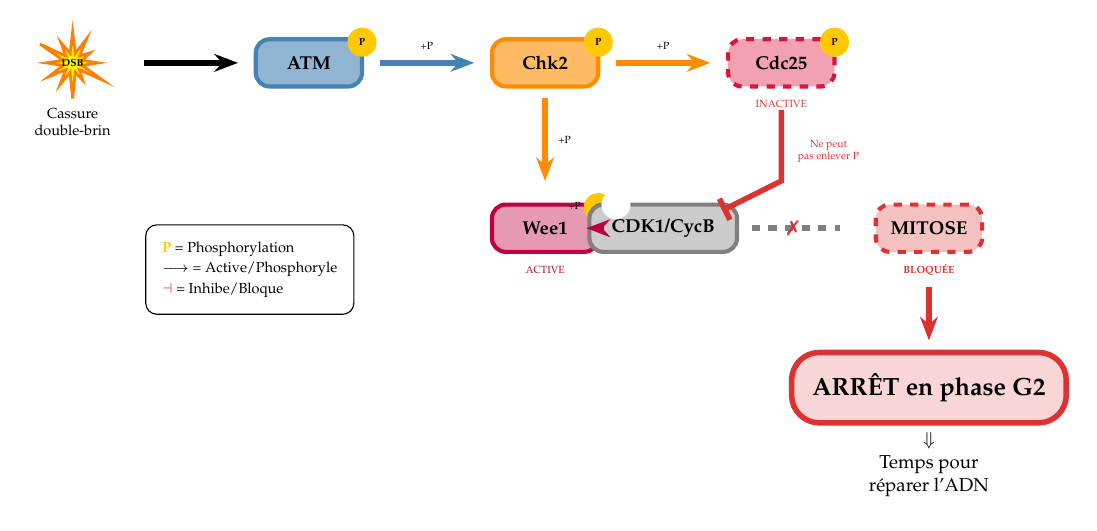
\begin{tikzpicture}[
    scale=0.75, 
    transform shape,
    box/.style={rectangle, rounded corners=5pt, minimum width=1.8cm, minimum height=0.8cm, line width=1.5pt, font=\small\bfseries, align=center},
    arrow/.style={-{Stealth[length=3mm]}, line width=2pt},
    inhibit/.style={-{Bar[width=3mm]}, line width=2pt, stopcolor}
]
    
    % === Dommage ADN ===
    \node[starburst, starburst points=12, fill=yellow, minimum size=1.2cm, draw=orange, line width=1pt] (dsb) at (0, 0) {};
    \node[font=\tiny\bfseries] at (0, 0) {DSB};
    \node[font=\scriptsize, align=center] at (0, -1) {Cassure\\double-brin};
    
    % Flèche vers ATM
    \draw[arrow, black] (1.2, 0) -- (2.8, 0);
    
    % === ATM ===
    \node[box, fill=atmcolor!60, draw=atmcolor] (atm) at (4, 0) {ATM};
    \node[circle, fill=phosphocolor, minimum size=0.35cm, font=\tiny\bfseries] at (4.9, 0.35) {P};
    
    % Flèche ATM vers Chk2
    \draw[arrow, atmcolor] (5.2, 0) -- (6.8, 0);
    \node[font=\tiny, above] at (6, 0.1) {+P};
    
    % === Chk2 ===
    \node[box, fill=chk2color!60, draw=chk2color] (chk2) at (8, 0) {Chk2};
    \node[circle, fill=phosphocolor, minimum size=0.35cm, font=\tiny\bfseries] at (8.9, 0.35) {P};
    
    % Flèche Chk2 vers Cdc25
    \draw[arrow, chk2color] (9.2, 0) -- (10.8, 0);
    \node[font=\tiny, above] at (10, 0.1) {+P};
    
    % === Cdc25 (inactivée) ===
    \node[box, fill=cdc25color!40, draw=cdc25color, dashed] (cdc25) at (12, 0) {Cdc25};
    \node[circle, fill=phosphocolor, minimum size=0.35cm, font=\tiny\bfseries] at (12.9, 0.35) {P};
    \node[font=\tiny, stopcolor] at (12, -0.7) {INACTIVE};
    
    % Inhibition de Wee1 par Chk2
    \draw[arrow, chk2color] (8, -0.6) -- (8, -2);
    \node[font=\tiny, right] at (8.1, -1.3) {+P};
    
    % === Wee1 (activée) ===
    \node[box, fill=purple!40, draw=purple] (wee1) at (8, -2.8) {Wee1};
    \node[circle, fill=phosphocolor, minimum size=0.35cm, font=\tiny\bfseries] at (8.9, -2.45) {P};
    \node[font=\tiny, purple] at (8, -3.5) {ACTIVE};
    
    % === CDK1/CycB ===
    \node[box, fill=gray!40, draw=gray, minimum width=2.5cm] (cdk1) at (10, -2.8) {CDK1/CycB};
    
    % Flèche Wee1 ajoute P sur CDK1
    \draw[arrow, purple] (9, -2.8) -- (8.7, -2.8);
    \node[circle, fill=stopcolor, minimum size=0.3cm, font=\tiny\bfseries, white] at (9.2, -2.4) {P};
    \node[font=\tiny, above] at (8.5, -2.6) {+P};
    
    % Cdc25 ne peut pas enlever P
    \draw[inhibit] (12, -0.8) -- (12, -2) -- (11, -2.5);
    \node[font=\tiny, stopcolor, align=center] at (12.8, -1.5) {Ne peut\\pas enlever P};
    
    % Flèche vers mitose bloquée
    \draw[line width=2pt, gray, dashed] (11.5, -2.8) -- (13, -2.8);
    \node[font=\normalsize, stopcolor] at (12.2, -2.8) {\ding{55}};
    
    % === Mitose ===
    \node[box, fill=stopcolor!30, draw=stopcolor, dashed] (mitose) at (14.5, -2.8) {MITOSE};
    \node[font=\tiny\bfseries, stopcolor] at (14.5, -3.5) {BLOQUÉE};
    
    % === Légende ===
    \node[draw, rectangle, rounded corners, fill=white, inner sep=8pt, font=\scriptsize, align=left] at (3, -3.5) {
        \textcolor{phosphocolor}{\textbf{P}} = Phosphorylation\\[2pt]
        $\longrightarrow$ = Active/Phosphoryle\\[2pt]
        \textcolor{stopcolor}{$\dashv$} = Inhibe/Bloque
    };
    
    % === ARRÊT G2 ===
    \node[draw, rectangle, rounded corners=10pt, fill=stopcolor!20, line width=2pt, draw=stopcolor, inner sep=10pt] at (14.5, -5.5) {
        \textbf{\large ARRÊT en phase G2}
    };
    \draw[arrow, stopcolor] (14.5, -3.8) -- (14.5, -4.7);
    
    % Temps pour réparation
    \node[font=\small, align=center] at (14.5, -6.8) {$\Downarrow$\\Temps pour\\réparer l'ADN};
    
\end{tikzpicture}
\caption{\textbf{Cascade complète de signalisation ATM.} Les DSB activent ATM, qui phosphoryle Chk2. Chk2 a deux effets : (1) il inactive Cdc25 (qui ne peut plus activer CDK1), et (2) il active Wee1 (qui maintient CDK1 inactif en le phosphorylant). Résultat : CDK1/Cycline B reste inactif et la mitose est bloquée.}
\end{figure}

%==============================================================================
% ANALOGIE
%==============================================================================
\section{Analogie : La voiture}

\begin{figure}[h!]
\centering
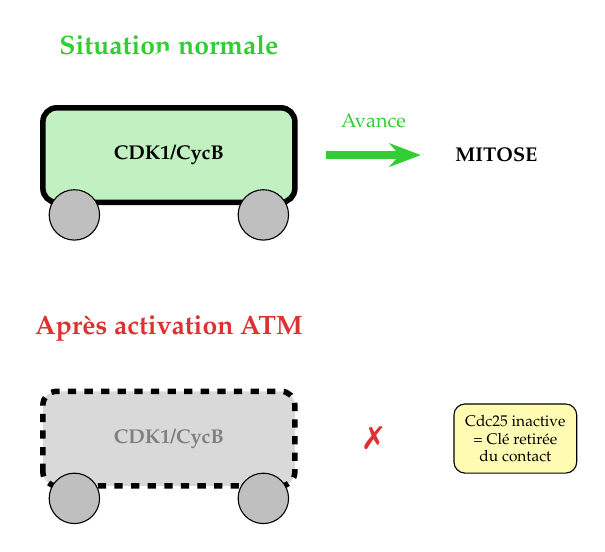
\begin{tikzpicture}[scale=0.8, transform shape]
    
    % === VOITURE NORMALE ===
    \node[font=\large\bfseries, gocolor] at (-4, 3) {Situation normale};
    
    % Voiture
    \draw[fill=gocolor!30, rounded corners=5pt, line width=2pt] (-6, 0.5) rectangle (-2, 2);
    \draw[fill=gray!50] (-5.5, 0.3) circle (0.4);
    \draw[fill=gray!50] (-2.5, 0.3) circle (0.4);
    \node[font=\small\bfseries] at (-4, 1.25) {CDK1/CycB};
    
    % Moteur ON
    \node[draw, circle, fill=gocolor, minimum size=0.8cm, font=\tiny\bfseries, white] at (-4, 2.5) {ON};
    
    % Flèche mouvement
    \draw[-{Stealth[length=4mm]}, line width=3pt, gocolor] (-1.5, 1.25) -- (0, 1.25);
    \node[font=\small, gocolor] at (-0.75, 1.8) {Avance};
    
    % Destination
    \node[font=\small\bfseries] at (1.2, 1.25) {MITOSE};
    
    % === VOITURE BLOQUÉE ===
    \node[font=\large\bfseries, stopcolor] at (-4, -1.5) {Après activation ATM};
    
    % Voiture
    \draw[fill=gray!30, rounded corners=5pt, line width=2pt, dashed] (-6, -4) rectangle (-2, -2.5);
    \draw[fill=gray!50] (-5.5, -4.2) circle (0.4);
    \draw[fill=gray!50] (-2.5, -4.2) circle (0.4);
    \node[font=\small\bfseries, gray] at (-4, -3.25) {CDK1/CycB};
    
    % Moteur OFF
    \node[draw, circle, fill=stopcolor, minimum size=0.8cm, font=\tiny\bfseries, white] at (-4, -2) {OFF};
    
    % Pas de mouvement
    \node[font=\Large, stopcolor] at (-0.75, -3.25) {\ding{55}};
    
    % Clé retirée = Cdc25 inactive
    \node[draw, rectangle, rounded corners, fill=yellow!30, inner sep=5pt, font=\scriptsize, align=center] at (1.5, -3.25) {
        Cdc25 inactive\\= Clé retirée\\du contact
    };
    
\end{tikzpicture}
\caption{\textbf{Analogie de la voiture.} CDK1/Cycline B est comme le moteur d'une voiture. Cdc25 est comme la clé de contact qui démarre le moteur. Quand ATM est activée, Cdc25 est ``retirée'' (inactivée) : le moteur ne peut pas démarrer et la voiture (cellule) ne peut pas avancer vers la mitose.}
\end{figure}

%==============================================================================
% RÉSUMÉ
%==============================================================================
\section{Résumé}

\begin{tcolorbox}[colback=atmcolor!10, colframe=atmcolor, title=\textbf{Points clés à retenir}]
\begin{enumerate}
    \item \textbf{Cascade = réaction en chaîne} : ATM $\rightarrow$ Chk2 $\rightarrow$ Cdc25 (inactive) $\dashv$ CDK1
    
    \item \textbf{Phosphorylation = interrupteur} : Ajouter un phosphate change l'activité d'une protéine (ON $\leftrightarrow$ OFF)
    
    \item \textbf{CDK1/Cycline B = moteur} : Ce complexe est indispensable pour déclencher la mitose
    
    \item \textbf{Cdc25 = clé de contact} : Normalement, Cdc25 active CDK1 en enlevant ses phosphates inhibiteurs
    
    \item \textbf{ATM = système de freinage d'urgence} : En inactivant Cdc25, ATM empêche le démarrage du ``moteur''
\end{enumerate}
\end{tcolorbox}

\vspace{0.5cm}

\begin{center}
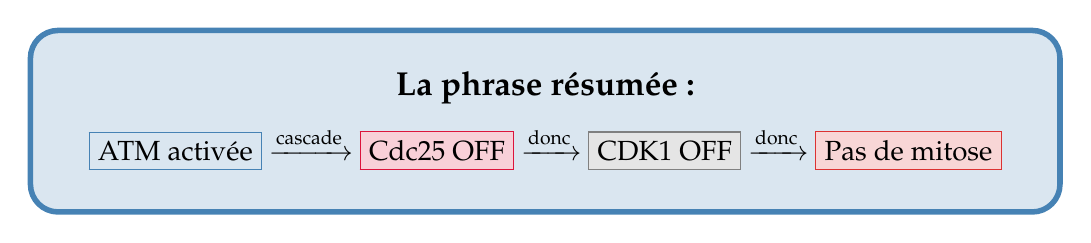
\begin{tikzpicture}
    \node[rectangle, rounded corners=10pt, fill=atmcolor!20, draw=atmcolor, line width=2pt, inner sep=15pt] {
        \begin{tabular}{c}
        \textbf{\large La phrase résumée :}\\[8pt]
        \fcolorbox{atmcolor}{atmcolor!20}{ATM activée} 
        $\xrightarrow{\text{cascade}}$ 
        \fcolorbox{cdc25color}{cdc25color!20}{Cdc25 OFF} 
        $\xrightarrow{\text{donc}}$ 
        \fcolorbox{gray}{gray!20}{CDK1 OFF} 
        $\xrightarrow{\text{donc}}$ 
        \fcolorbox{stopcolor}{stopcolor!20}{Pas de mitose}
        \end{tabular}
    };
\end{tikzpicture}
\end{center}

\end{document}
